\begin{itemize}
\item \begin{tabular}{|l|l|}
\hline
$x$ & $x^2$\\
\hline
1 & 1\\
\hline
2 & 4\\
\hline
3 & 9\\
\hline
4 & 16\\
\hline
5 & 25\\
\hline
6 & 36\\
\hline
7 & 49\\
\hline
8 & 64\\
\hline
9 & 81\\
\hline
\end{tabular}
\item \begin{itemize}
\item Let's output an identity matrix
\item \begin{tabular}{ l l l l l }

1 & 0 & 0 & 0 & 0\\

0 & 1 & 0 & 0 & 0\\

0 & 0 & 1 & 0 & 0\\

0 & 0 & 0 & 1 & 0\\

0 & 0 & 0 & 0 & 1\\

\end{tabular}
\item \begin{enumerate}
\item PyTex can use this way to create a latex document
\item And we can also create new filed using program
\item For example, the next 10 line are 10 random number generated by python
\item the 0-th random number is 0.351207629222
\item the 1-th random number is 0.74917531364
\item the 2-th random number is 0.553320911684
\item the 3-th random number is 0.495962106322
\item the 4-th random number is 0.582170842076
\item the 5-th random number is 0.472835037611
\item the 6-th random number is 0.752803670144
\item the 7-th random number is 0.353354513795
\item the 8-th random number is 0.525044538949
\item the 9-th random number is 0.982742002199
\end{enumerate}
\item let's try a plot
\item 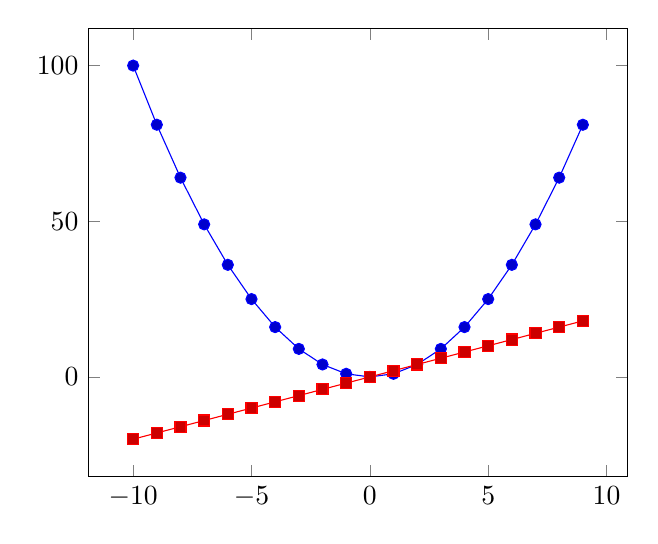
\begin{tikzpicture}
\begin{axis}
\addplot coordinates {
(-10,100)
(-9,81)
(-8,64)
(-7,49)
(-6,36)
(-5,25)
(-4,16)
(-3,9)
(-2,4)
(-1,1)
(0,0)
(1,1)
(2,4)
(3,9)
(4,16)
(5,25)
(6,36)
(7,49)
(8,64)
(9,81)
};
\addplot coordinates {
(-10,-20)
(-9,-18)
(-8,-16)
(-7,-14)
(-6,-12)
(-5,-10)
(-4,-8)
(-3,-6)
(-2,-4)
(-1,-2)
(0,0)
(1,2)
(2,4)
(3,6)
(4,8)
(5,10)
(6,12)
(7,14)
(8,16)
(9,18)
};
\end{axis}
\end{tikzpicture}
\end{itemize}
\end{itemize}
